\section{Architecture Design \& Implementation}
\subsection{Overall architecture}

\begin{figure}[htb]
\centerline{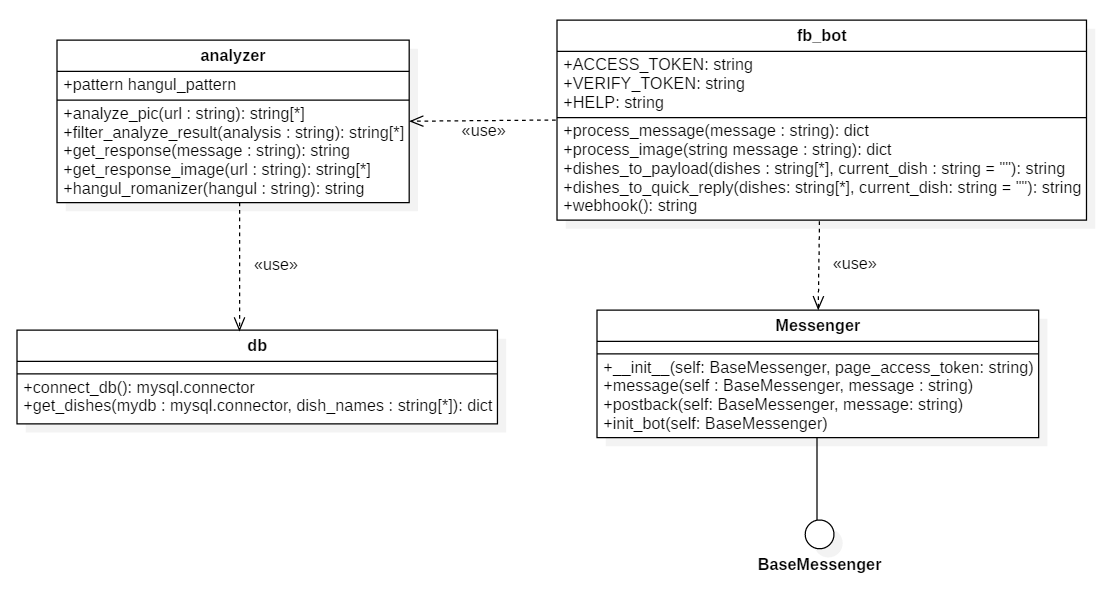
\includegraphics[width=\linewidth]{./pictures/uml}}
\caption{UML of our overall architecture}
\label{fig:uml}
\end{figure}
\FloatBarrier

\subsection{Directory organization}

\begin{table}[htbp]
\caption{Directory organization}
\begin{tabularx}{\linewidth}{|X|X|X|}
\toprule
Directory & File names & Module names in use  \\
\midrule
./src & messenger.py & messenger  \newline\\
./src & fb\_bot.py &  fb\_bot\newline \\
./src & ssl\_certificate.pem db.py \newline  & db \\
./src & analyzer.py & analyzer \newline \\
./tests & 
test.txt \newline 
test\_db.py \newline
test\_json.py	 \newline
test.jpg  \newline
& test\\
./db & food.mwb \newline & db model  \\
./doc & before\_order.tex before\_order.pdf \newline & documentation  \\
./doc/content & architecture\_design\_a nd\_implementation.tex development\_environ ment.tex introduction.tex requirements.tex specifications.tex use\_cases.tex Installation\_guide.tex discussion.tex \newline & documentation \\
./doc/pictures & 
facebook\_dish\_info.png \newline
facebook\_friends.png \newline
facebook\_meun.png \newline
facebook\_message.png \newline
facebook\_overview.png \newline
facebook\_profil.png \newline
facebook\_response.png \newline
facebook\_response\_sele ction.png\newline
uml.png \newline
class\_uml.mdj \newline
facebook\_search\_chatbot.png \newline
facebook\_initial\_page.png \newline
facebook\_input\_selection.png \newline
facebook\_user\_input.png \newline
facebook\_analysis.png \newline
facebook\_result.png \newline
facebook\_different\_expressions.png \newline
facebook\_additional\_feature.png \newline
facebook\_gif\_image.png
& documentation \\
\end{tabularx}
\end{table}
\FloatBarrier

\subsection{Module 1 - messenger} 

\begin{figure}[htbp]
\centerline{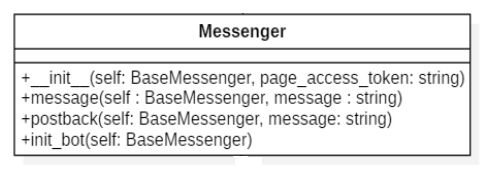
\includegraphics[width=\linewidth]{./pictures/class_messenger}}
\caption{Class Messenger}
\label{fig:class_messenger}
\end{figure}
\FloatBarrier

\subsubsection {Purpose}

The Facebook Messenger chatbot needs Facebook Messenger API to interact with the facebook users who need our service. This module can provides a connection with the Facebook Messenger API, so chatbot can send message to users and receive message from users through this module. It is the most important factor that allows the messenger to function.  

\subsubsection {Functionality}

This module makes chatbot be able to send messages to the users and receive messages from the users. There is a Facebook server between users and our chatbot server. Facebook provides a webhook function and it gives our chatbot server alerts that user sent a message to our chatbot or other user reaction to our chatbot (entering chatbot chatroom etc.) and messages. Through this module, we can give a response to users immediately and can provide our service. When users send messages, we can implement the appropriate chatbot action and build scenarios in which to communicate with users. It also provides the transmission of text as well as other extension files, such as pictures and files, to enable context-sensitive types of messages to be sent. 

\subsubsection {Location of Source Code}

/project/src


\subsubsection {Class component}

The messenger module has messenger class. It extends BaseMessenger class, that is provided from the fbmessenger package. fbmessenger is a python library to communicate with the Facebook Messenger API's. It provides various functionality and class to implement the chatbot service. The class doesnt have a variable and it has serveral methods for service. The methods that class has are as follows:

\begin{itemize}
\item \_\_init\_\_(self:BaseMessenger, page\_access\_token): constructor of the messenger class. it makes messegner object.
\item message(self: BaseMessenger, message): The message function is called when we get a "message" object from the webhook. The webhook can send a few different json messages, and we can specify which message types we want to receive when we set up the webhook. And message() is general when the user sends us a message. So in the message function, when we receive a message we first send an achknowledgment to the user that we received it and computing it. 
\item postback(self: BaseMessenger, message): This method can handle a postback webhook. The Facebook Messenger supports the postback meun for users. The users can invoke an action in our bot through the button. When users press the button to invoke some actions in cahtbot, chatbot receives a postback webhook from the Facebook Messenger server. This function can handle this webhook, so can give some responses to the user.
\item init\_bot(self: BaseMessenger): the init\_bot method initiate our chatbot. It initiate greetings and actions list that the users can select when they start our chatbot. And, it also provides customized buttons function that the users can choose during the scenario. 
\end{itemize} 

\FloatBarrier

\subsection{Module 2 - fb\_bot}


\begin{figure}[htbp]
\centerline{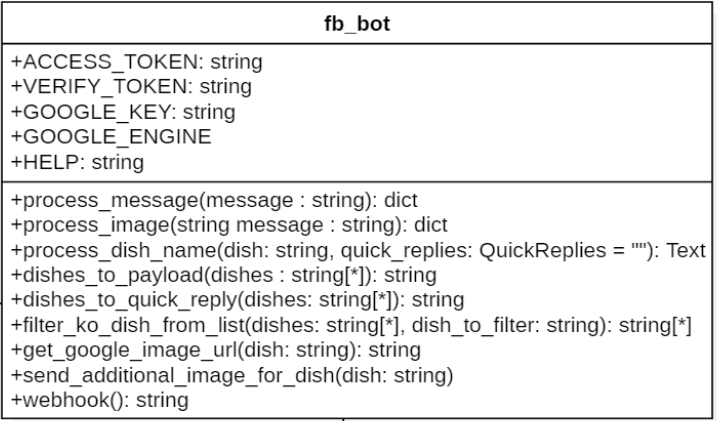
\includegraphics[width=\linewidth]{./pictures/class_fb_bot}}
\caption{Class fb\_bot}
\label{fig:class_fb_bot}
\end{figure}
\FloatBarrier


\subsubsection {Purpose}

We need an intermediary between our chatbot and functionality of our service. A module fb\_bot plays such a role. The module fb\_bot allows each module to be grouped and became a bridge that enables our services to be delivered to users.


\subsubsection {Functionality}

The fb\_bot module handles messages from the module messenger to reply to users. When the messenger gets text from the users, the module processes a message in condition of the text. If a messenger gets a picture type file from the users, the module fb\_bot calls a module analyzer to analyze picture that gets from user and get information of dishes from our database. And It process our data that is from module analyzer agian, and sends back to the module messenger to give results to the users. The module fb\_bot has several functionalties to interact with other modules.


\subsubsection {Location of Source Code}

/project/src


\subsubsection {Class component}

The class fb\_bot has three member variables. They are as follows:

\begin{itemize}
\item ACCESS\_TOKEN:string : ACCESS\_TOKEN is for accessing to the the chatbot messenger. Each chatbot has an unique ACCESS\_TOKEN. A module fb\_bot can get messages from the bot using the token. We need it everytime we send a message to facebook. 
\item VERIFY\_TOKEN:string : it is used when facebook senta a first message to check if the server exists. the VERIFY\_TOKEN can be anything we want to, we just have to specify it when setting up the webhook.
\item HELP:string : When user write 'help' or type some messages that is not related to request for our service, chatbot sents this string.
\end{itemize} 

The methods that class fb\_bot has are as follows:

\begin{itemize}
\item process\_message(message):dict : This method returns reply message based on the type of message sent by the user. There are several conditions in it, and it retuns specific reply that the user wants. It can be the scenario handler for our chatbot. I can handle all kinds of type of messages.
\item process\_image(message):dict : This method is only for the condition when user send picture type message that users want to know about. It calls analyzer method to get an infromation of dishes and returns description about dishes. It includes all the action messages while the picture analyzes and the information receives. In the action messages, the quick reply type message is included in here. 
\item dishes\_to\_payload(dishes, current\_dish):string : The method is used in the dishes\_to\_quick\_reply method. It saves dish list as a jason format.
\item dishes\_to\_quick\_reply(dishes, current\_dish):string : The method is for replying to quick reply message type. A quick reply message is one of the message type that Facebook Messenger supports, it consists of the button list. When the fb\_bot module gets dish list from the analyzer module, it creates the quick reply buttons for user to choose one of them to get a information. It calls dishes\_to\_payload method to save the list of dishes that it havent given yet to the users.
\item webhook():string : The webhook method controls the connection between Facebook Messeneger server and the chatbot server. It uses Flask, the microframework for python. It uses VERIFY\_TOKEN to check if the server exists. And if it exists, It initiates our chatbot service using init\_bot method in messenger module.
\end{itemize} 

\FloatBarrier


\subsection{Module 3 - analyzer}



\begin{figure}[htbp]
\centerline{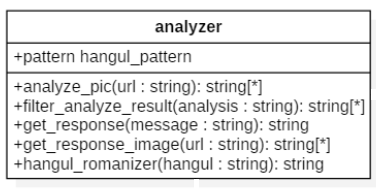
\includegraphics[width=\linewidth]{./pictures/class_analyzer}}
\caption{Class Analyzer}
\label{fig:class_analyzer}
\end{figure}
\FloatBarrier

\subsubsection {Purpose}

A module analyzer has an important role in our service. We need to extract korean letters from the picture, and find the dish names about which users want to know. Therefore, this module is necessary to analyze image. It linked with our main service function, Azure OCR Text Recognition API. And, it makes requests to get analysis results from it. It also serves final information that user wants. 

\subsubsection {Functionality}

The module analyzer processes image through the OCR Text Recongnition API to extract the text from the image. When it gets result from Recognition API, it searchs only krorean letters from the result. It becomes a list of the dishes that users want to know. Then analyzer sends a query to the db module to search description for that dish name. It also romanizes korean dish name to roman and provides the name with description to the fb\_bot.

\subsubsection {Location of Source Code}
/project/src

\subsubsection {Class component}


\begin{itemize}

\item pattern hangul\_pattern : The pattern is used to distinguish whether the text is hangul or not.
\item analyze\_pic(url):string[*] : The analyze\_pic() method checks the image url that comes from users is available, and sends request to the Azure OCR Text Recognition API. It needs specific json type input, so it organizes the format and returns result that is from the API.
\item filter\_analyze\_result(analysis):string[*] : The method filter analyze result() gets analysis as a parameter. This the return value of analyze\_pic() method. When it called, the method extracts only korean letters from the analysis string list. The pattern hangul\_pattern is used to distinguish korean letters from the list. 
\item get\_response(message):string : A get\_response method is called when user sends dish name. It calls db module to get information of dish from database server, and it combines dishe's korean name, its roman name and description. When it creates final description, it returns the description.
\item get\_response\_image(url):string[*] : The method is called when user sends picture of menu. It calls filter\_analyze\_result method to get the korean dishes list and it sends query to find information from the server. and it returns the description of dish.
\item hangul\_romanizer(hangul):string : The hangul romanizer method romanize dish name. it uses python library hangul\_romanize. It support Tarnsliter class and it just makes korean text to roman. 
\end{itemize} 

\FloatBarrier

\subsection{Module 4 - db}

\begin{figure}[htbp]
\centerline{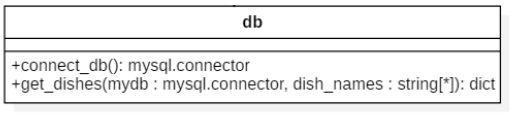
\includegraphics[width=\linewidth]{./pictures/class_db}}
\caption{Class db}
\label{fig:class_db}
\end{figure}
\FloatBarrier

\subsubsection {Purpose}

The module db is used to get information of dishes from the database server.   
\subsubsection {Functionality}

We have own MySQL database that stores description of the dishes. The module makes a connection with the MySQL database server and it can send queries to the database server and get a result of the query. 


\subsubsection {Location of Source Code}

/project/src

\subsubsection {Class component}

The class has no member variable, and the class methods are as follows:

\begin{itemize}
\item connect\_db():mysql.connector :  It makes a connector object to connect with our MySQL server to send the query to it. It includes the connection information to connect to database. It uses mysql.connector library to get the mysql.connector class. 

\item get\_dishes(mydb, dish\_names):dict : It sends a query for getting dishes information to the database server using the connector object. The query is for getting descriptions of specific dish name that the module analyzer gives as a parameter. And it returns the results from the database as dictionary. \newline\newline

\end{itemize}

\FloatBarrier

